% Created 2019-06-14 vie 18:11
% Intended LaTeX compiler: pdflatex
\documentclass[xcolor={usenames,svgnames,dvipsnames}]{beamer}
\usepackage[utf8]{inputenc}
\usepackage[T1]{fontenc}
\usepackage{graphicx}
\usepackage{grffile}
\usepackage{longtable}
\usepackage{wrapfig}
\usepackage{rotating}
\usepackage[normalem]{ulem}
\usepackage{amsmath}
\usepackage{textcomp}
\usepackage{amssymb}
\usepackage{capt-of}
\usepackage{hyperref}
\usepackage{color}
\usepackage{listings}
\usepackage[spanish]{babel}
\usecolortheme{rose}
\setbeamercolor{alerted text}{fg=Blue}
\setbeamerfont{alerted text}{series=\bfseries}
\setbeamerfont{block title}{series=\bfseries}
\setbeamercolor{block title}{bg=structure.fg!20!bg!50!bg}
\setbeamercolor{block body}{use=block title,bg=block title.bg}
\setbeamertemplate{navigation symbols}{}
\AtBeginSection[]{\begin{frame}[plain]\tableofcontents[currentsection,sectionstyle=show/shaded, subsectionstyle=show/hide]\end{frame}}
\AtBeginSubsection[]{\begin{frame}[plain]\tableofcontents[currentsubsection,sectionstyle=show/shaded,subsectionstyle=show/shaded/hide]\end{frame}}
\lstset{keywordstyle=\color{blue}, commentstyle=\color{gray!90}, basicstyle=\ttfamily\small, columns=fullflexible, breaklines=true,linewidth=\textwidth, backgroundcolor=\color{gray!23}, basewidth={0.5em,0.4em}, literate={¡}{{\textexclamdown}}1 {á}{{\'a}}1 {ñ}{{\~n}}1 {é}{{\'e}}1 {ó}{{\'o}}1 {í}{{\'i}}1 {ú}{{\'u}}1 {º}{{\textordmasculine}}1, showstringspaces=false}
\usepackage{mathpazo}
\hypersetup{colorlinks=true, linkcolor=Blue, urlcolor=Blue}
\usepackage{fancyvrb}
\DefineVerbatimEnvironment{verbatim}{Verbatim}{fontsize=\tiny, formatcom = {\color{black!70}}}
\beamertemplatenavigationsymbolsempty
\setbeamertemplate{footline}[frame number]
\usetheme{Boadilla}
\usefonttheme{serif}
\author{Oscar Perpiñán Lamigueiro}
\date{}
\title{Introducción al control de versiones y trabajo colaborativo con GitHub}
\hypersetup{
 pdfauthor={Oscar Perpiñán Lamigueiro},
 pdftitle={Introducción al control de versiones y trabajo colaborativo con GitHub},
 pdfkeywords={},
 pdfsubject={},
 pdfcreator={Emacs 26.1 (Org mode 9.2)}, 
 pdflang={Spanish}}
\begin{document}

\maketitle

\begin{frame}[label={sec:org5c5baf9}]{AIGORA}
Lo expuesto en este documento se enmarca en el proyecto de innovación educativa AIGORA (Aprendizaje de Informática con Github Organizado en Repositorios Abiertos).

\begin{center}

\includegraphics[height=0.5\textheight]{figs/aigora.png}
\end{center}

\url{https://innovacioneducativa.upm.es/proyectosIE/informacion?anyo=2018-2019\&id=2840}
\end{frame}

\section{Conceptos básicos}
\label{sec:org70b7969}
\subsection{¿Qué es el control de versiones?}
\label{sec:orgf5cd0c0}

\begin{frame}[label={sec:org877d3f9},plain]{}
\begin{center}

\includegraphics[width=0.9\paperwidth]{figs/phdcomic_finaldoc_1.png}
\end{center}

\url{http://phdcomics.com/comics/archive.php?comicid=1531}
\end{frame}

\begin{frame}[label={sec:org57fd6e1},plain]{}
\begin{center}

\includegraphics[width=0.9\paperwidth]{figs/phdcomic_finaldoc_2.png}
\end{center}

\url{http://phdcomics.com/comics/archive.php?comicid=1531}
\end{frame}

\begin{frame}[label={sec:org3fa6fa2},plain]{}
\begin{center}

\includegraphics[width=0.9\paperwidth]{figs/phdcomic_finaldoc_3.png}
\end{center}

\url{http://phdcomics.com/comics/archive.php?comicid=1531}
\end{frame}

\begin{frame}[label={sec:org748a067}]{¿Qué es el control de versiones y por qué debería importarte?}
\begin{quote}
El control de versiones es un sistema que \alert{registra los cambios}
realizados sobre un archivo o conjunto de archivos a lo largo del
tiempo, de modo que se puedan \alert{recuperar} versiones específicas más
adelante.\footnote{\url{https://git-scm.com/book/es/v1/Empezando-Acerca-del-control-de-versiones}}
\end{quote}
\begin{block}{Viajar en el tiempo}
\begin{itemize}
\item Nada que haya sido sometido a un control de versiones se pierde jamás (\emph{salvo que realmente quieras eliminarlo\ldots{}})
\item \alert{Todas} las versiones antiguas de un fichero se almacenan: un fichero se puede revertir a un estado anterior sin límites.
\end{itemize}
\end{block}
\end{frame}
\begin{frame}[label={sec:org2c81d02}]{¿Qué es el control de versiones y por qué debería importarte?}
\begin{quote}
El control de versiones es el \alert{cuaderno de laboratorio} en el mundo digital. Es lo que los profesionales usan para realizar un
\alert{seguimiento} de lo que han hecho y para \alert{colaborar} con otras
personas.\footnote{\url{https://swcarpentry.github.io/git-novice/}\label{orge30ca7c}}
\end{quote}


\begin{block}{¿Qué? ¿Cuándo? ¿Quién?}
Un sistema de control de versiones registra:
\begin{itemize}
\item El detalle de los cambios realizados.
\item La fecha y hora en la que fueron realizados.
\item La persona que los realizó.
\end{itemize}
\end{block}
\end{frame}

\begin{frame}[label={sec:org59381cf}]{¿Qué es el control de versiones y por qué debería importarte?}
\begin{quote}
El control de versiones es el \alert{cuaderno de laboratorio} en el mundo digital. Es lo que los profesionales usan para realizar un
\alert{seguimiento} de lo que han hecho y para \alert{colaborar} con otras
personas.\textsuperscript{\ref{orge30ca7c}}
\end{quote}

\begin{block}{Trabajo Colaborativo}
\begin{itemize}
\item Cuando un equipo de personas trabaja conjuntamente en un proyecto, es posible que se produzcan cambios incompatibles en un mismo fichero.
\item El sistema de control de versiones \alert{impide} cambios simultáneos en un fichero. A cambio, permite la \alert{resolución de conflictos} y los documenta.
\end{itemize}
\end{block}
\end{frame}

\begin{frame}[label={sec:orgdb0d6ff}]{¿Qué es el control de versiones y por qué debería importarte?}
\begin{quote}
\alert{No sirve sólo para software}: libros, documentos, pequeños conjuntos
de datos y cualquier cosa que cambie con el tiempo o que deba
compartirse puede y debe almacenarse en un sistema de control de
versiones.\textsuperscript{\ref{orge30ca7c}}
\end{quote}
\end{frame}

\subsection{¿Qué son Git y GitHub?}
\label{sec:org6dd5e46}

\begin{frame}[label={sec:orgf661adf},fragile]{Git es un Sistema de Control de Versiones}
 Git es una herramienta software (accesible mediante línea de comandos con \texttt{git}) que implementa un Sistema de Control de Versiones.

\begin{center}
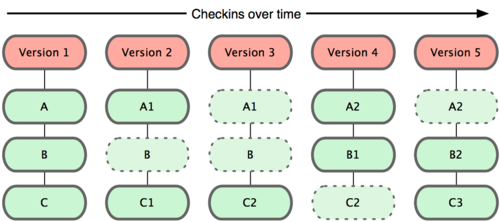
\includegraphics[width=.9\linewidth]{figs/git_model.png}
\end{center}
\end{frame}

\begin{frame}[label={sec:org10ee6fb}]{Git es un Sistema de Control de Versiones}
Cada vez que se ejecuta un cambio en una estructura de ficheros controlada con Git, realiza una \guillemotleft{}foto\guillemotright{} del estado de los archivos en ese momento, y guarda una referencia a esa instantánea. 
\begin{center}
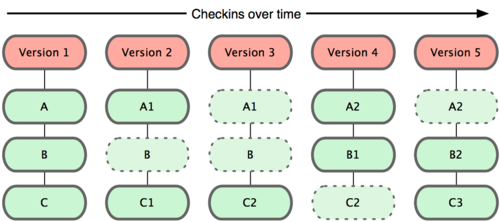
\includegraphics[width=.9\linewidth]{figs/git_model.png}
\end{center}
\end{frame}

\begin{frame}[label={sec:org008b985}]{Git es un Sistema de Control de Versiones}
Por eficiencia, Git no almacena los archivos sin modificaciones sino un enlace al archivo anterior idéntico que ya está almacenado

\begin{center}
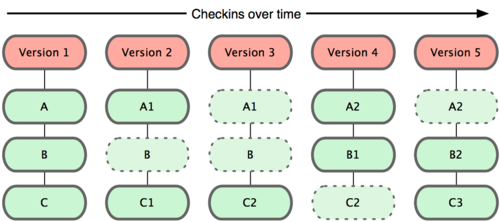
\includegraphics[width=.9\linewidth]{figs/git_model.png}
\end{center}
\end{frame}

\begin{frame}[label={sec:org5e0e73c}]{Los estados de Git}
\begin{itemize}
\item El desarrollador incorpora uno o varios ficheros al control de versiones. (\emph{tracked})
\item Realiza modificaciones en los ficheros (\emph{modified}).
\item Incorpora esos ficheros modificados al área de preparación (\emph{staged}).
\item Finalmente, confirma todos los cambios del área de preparación: se realiza la instantánea de los ficheros. (\emph{committed})
\end{itemize}
\begin{center}
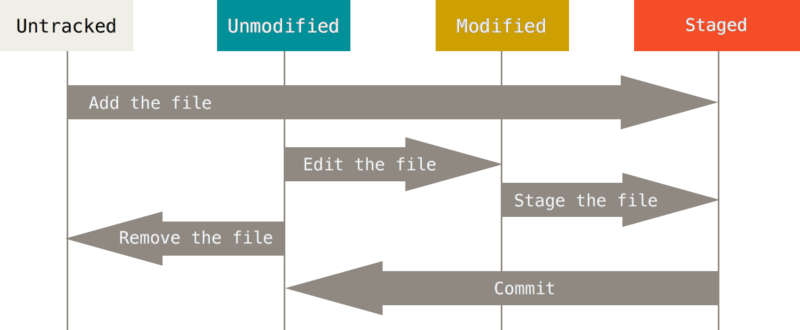
\includegraphics[height=0.4\textheight]{figs/git_estados.png}
\end{center}
\end{frame}

\begin{frame}[label={sec:org228bc95},fragile]{¿Qué es GitHub?}
 \begin{itemize}
\item GitHub es la plataforma de alojamiento de código más importante a nivel mundial.
\item Emplea el sistema de control de versiones \texttt{git}
\item Ofrece una amplia variedad de funcionalidades
\begin{itemize}
\item Alojamiento de código
\item Revisión de código
\item Trabajo colaborativo
\item Publicación de páginas web
\end{itemize}
\end{itemize}
\end{frame}

\section{Uso de \texttt{git} y \texttt{GitHub}}
\label{sec:org2e60237}

\subsection{Primeros Pasos}
\label{sec:orgecdaeed}
\begin{frame}[label={sec:org9728a7c}]{Creación de una cuenta en GitHub}
\url{https://github.com/join}

\begin{center}
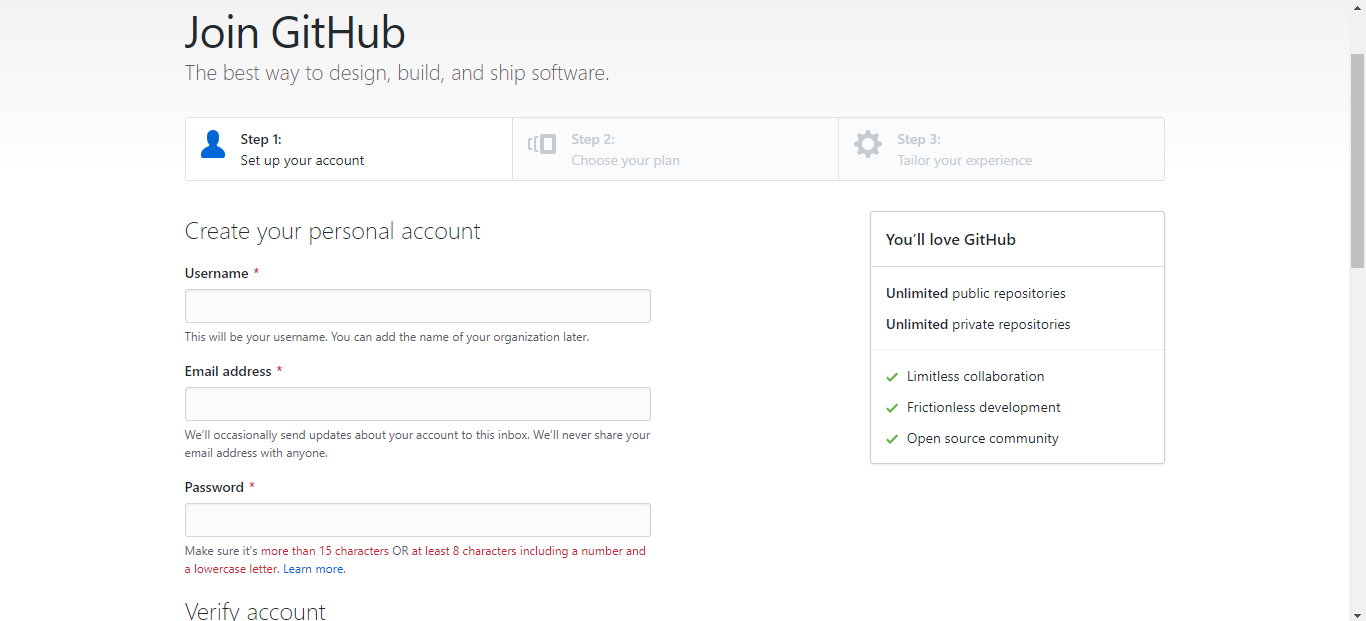
\includegraphics[width=.9\linewidth]{figs/GitHub_Join.png}
\end{center}

Más información en \href{https://help.github.com/articles/signing-up-for-a-new-github-account/}{New GitHub account}
\end{frame}

\begin{frame}[label={sec:orgbaacff4}]{Instalación de GitHub Desktop}
\url{https://desktop.github.com/}

\begin{center}

\includegraphics[width=.9\linewidth]{figs/GitHub_Desktop.png}
\end{center}
\end{frame}

\begin{frame}[label={sec:orgd32c494}]{Conectamos Git, GitHub y GitHub Desktop}
\begin{itemize}
\item Una vez instalado comienza el proceso de autenticación, usando las credenciales del paso anterior\footnote{Más información en \href{https://help.github.com/desktop/guides/getting-started-with-github-desktop/authenticating-to-github/}{Authenticating to GitHub}.}.
\end{itemize}

\begin{center}
\boxed{File > Options > Accounts > Sign\ In}
\end{center}


\begin{itemize}
\item A continuación, conectamos la información de usuario con Git\footnote{Más información en \href{https://help.github.com/desktop/guides/getting-started-with-github-desktop/configuring-git-for-github-desktop/}{Configuring Git}.}.
\end{itemize}

\begin{center}
\boxed{File > Options > Git}
\end{center}
\end{frame}

\begin{frame}[label={sec:orgc005986}]{}
\begin{block}{Ejercicio}
Abre una cuenta en GitHub, empleando el correo electrónico de la UPM (será útil más tarde, al usar GitHub Classroom), y configura GitHub Desktop para usar esta cuenta.
\end{block}
\end{frame}

\begin{frame}[label={sec:org046460d},fragile]{Remoto y Local}
 \begin{itemize}
\item \alert{Github.com} aloja los \alert{repositorios remotos} (nube).
\item En tu ordenador trabajas con una \alert{copia local} del repositorio. Otros desarrolladores tendrán sus propias copias locales.
\item La(s) copia(s) local(es) y el repositorio remoto deben estar \alert{sincronizados} mediante diferentes comandos de \texttt{git}.
\end{itemize}
\end{frame}
\begin{frame}[label={sec:orga760d74}]{Nuevo repositorio \emph{remoto} desde github.com}
\url{https://github.com/new}

\begin{center}
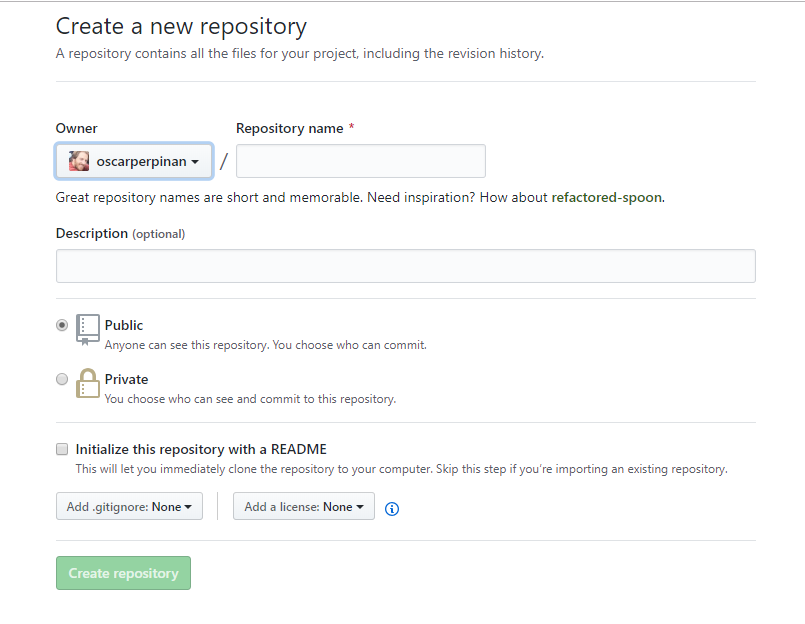
\includegraphics[width=.9\linewidth]{figs/GitHub_New_Repository.png}
\end{center}
\end{frame}

\begin{frame}[label={sec:org8fbbf64}]{Nuevo repositorio \emph{local} desde GitHub Desktop}
\begin{center}
\boxed{File > New\ Repository}
\end{center}

\begin{center}
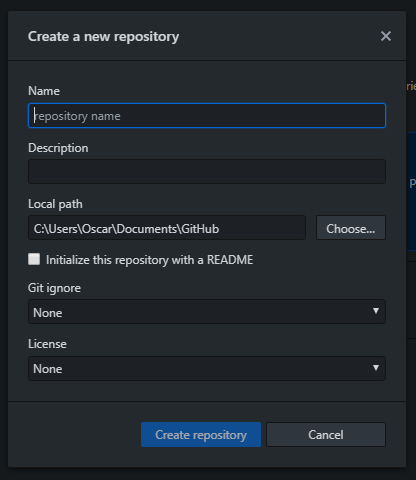
\includegraphics[height=0.7\textheight]{figs/Desktop_NewRepository.png}
\end{center}
\end{frame}

\begin{frame}[label={sec:orgef70bcc},fragile]{Decisiones al crear un repositorio}
 \begin{itemize}
\item Elige un \alert{\texttt{.gitignore}} adecuado al proyecto: Veáse \url{https://github.com/github/gitignore}.
\item No olvides inicializar y cumplimentar el \alert{\texttt{README.md}}. Para el formato veáse \href{https://help.github.com/articles/basic-writing-and-formatting-syntax/}{Formatting syntax}.
\item Elige una \alert{licencia} adecuada a tu proyecto y a tus intereses actuales y futuros. Veáse \url{https://choosealicense.com}.
\end{itemize}
\end{frame}

\begin{frame}[label={sec:orgf3aec4c}]{Clonar un repositorio remoto}
Si hemos creado el repositorio desde github.com (\emph{repositorio remoto}), hay que clonarlo para poder trabajar con él (\emph{copia local}).

\begin{center}
\boxed{File > Clone\ Repository}
\end{center}

\begin{center}
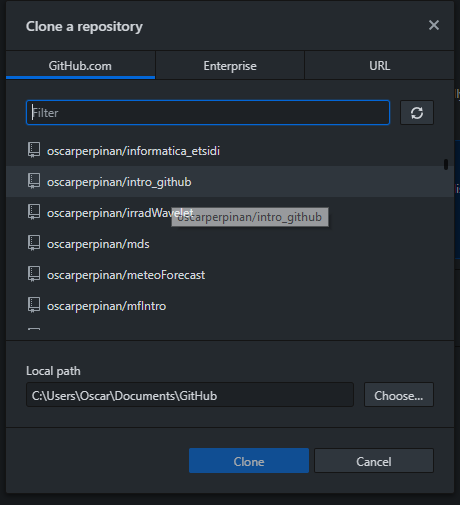
\includegraphics[height=0.65\textheight]{figs/Desktop_CloneRepository.png}
\end{center}
\end{frame}

\begin{frame}[label={sec:org8b6ac78}]{Publicar un repositorio local}
Si hemos creado el repositorio desde GitHub Desktop (\emph{repositorio local}), hay que publicarlo en github.com (\emph{repositorio remoto})

\begin{center}
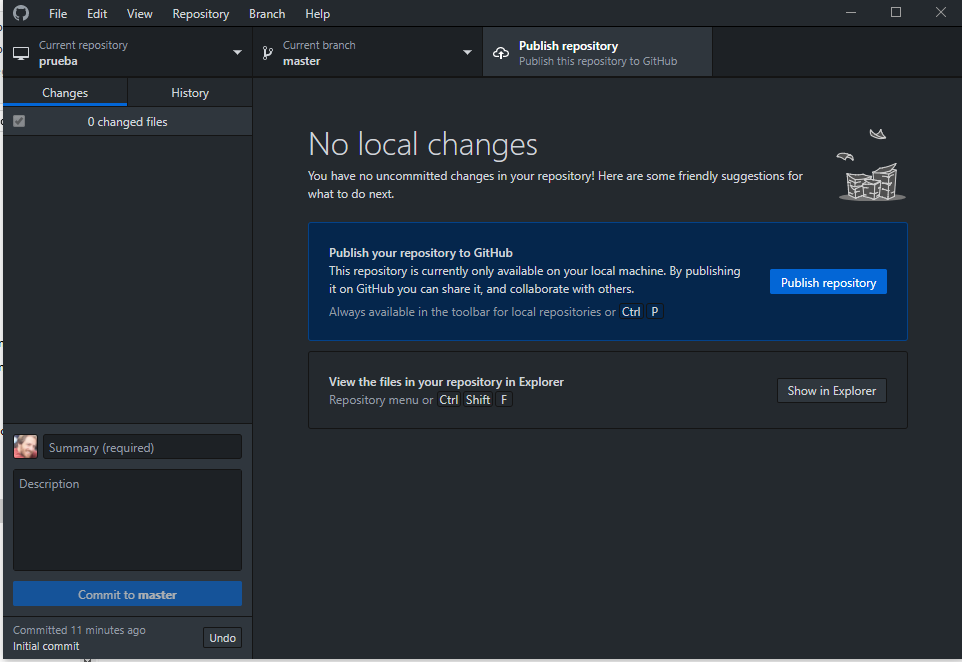
\includegraphics[width=.9\linewidth]{figs/Desktop_PublishRepository.png}
\end{center}
\end{frame}

\begin{frame}[label={sec:org5933be6},fragile]{}
 \begin{block}{Ejercicio}
Crea un nuevo repositorio remoto y haz la clonación del mismo para tener una copia local. No olvides elegir la licencia, generar una \texttt{README} y un \texttt{.gitignore}.
\end{block}
\end{frame}
\subsection{Flujo de Trabajo}
\label{sec:orgc1a5890}
\begin{frame}[label={sec:orge0d17f5}]{}
\begin{center}
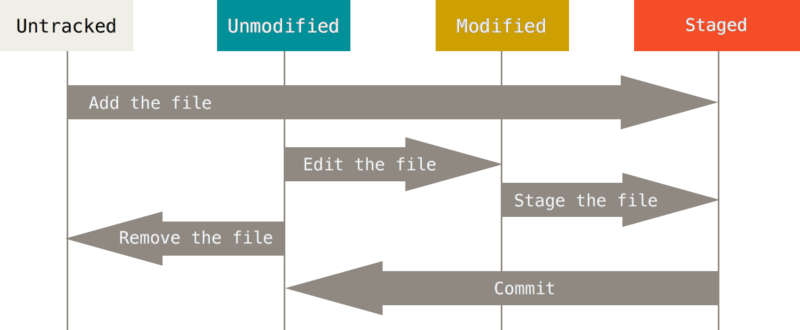
\includegraphics[width=.9\linewidth]{figs/git_estados.png}
\end{center}
\end{frame}

\begin{frame}[label={sec:org68d70b9}]{Cambios en la copia local}
\begin{center}
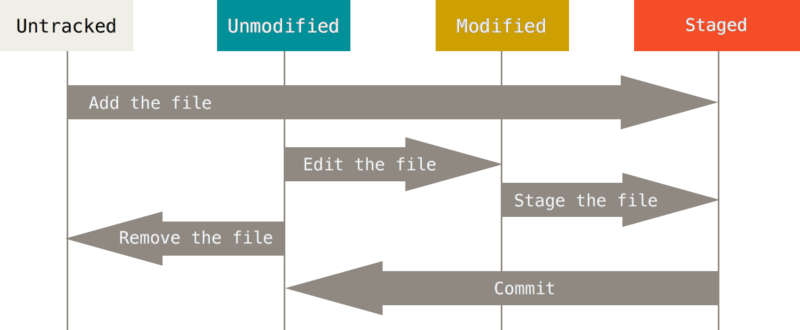
\includegraphics[height=0.4\textheight]{figs/git_estados.png}
\end{center}

En la carpeta que contiene la copia local, haz \alert{modificaciones} en los ficheros (empleando tu editor de código/texto preferido).
\end{frame}

\begin{frame}[label={sec:orgcb1fb9e},fragile]{Cambios en la copia local}
 \begin{center}
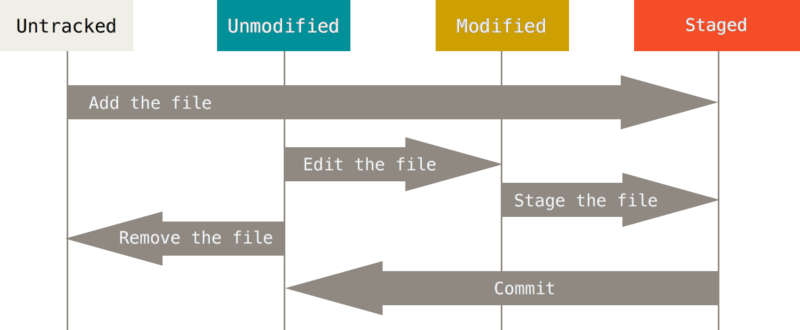
\includegraphics[height=0.4\textheight]{figs/git_estados.png}
\end{center}

\alert{Añade los cambios} realizados a la siguiente \guillemotleft{}instantánea\guillemotright{} del repositorio (\texttt{git add}) \begin{center}
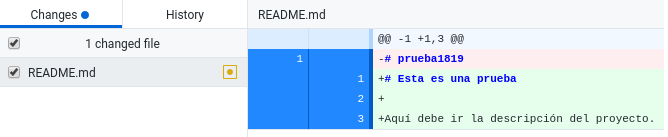
\includegraphics[width=.9\linewidth]{figs/git_add.png}
\end{center}
\end{frame}
\begin{frame}[label={sec:org71fcb69},fragile]{Cambios en la copia local}
 \begin{center}
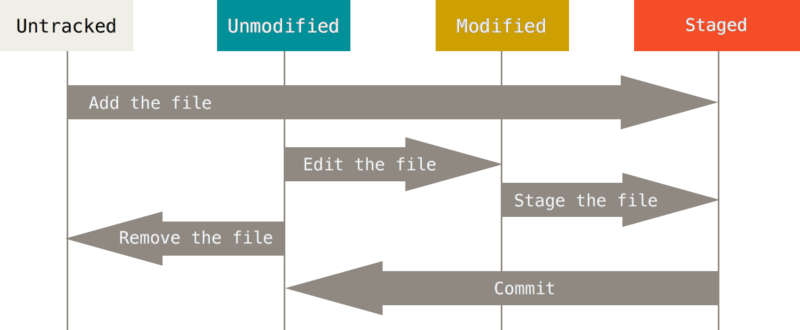
\includegraphics[height=0.4\textheight]{figs/git_estados.png}
\end{center}

\alert{Confirma} los cambios, escribiendo un resumen de lo realizado (\texttt{git commit})
\begin{center}
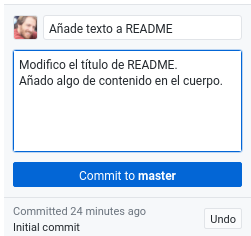
\includegraphics[height=0.3\textheight]{figs/git_commit.png}
\end{center}
\end{frame}
\begin{frame}[label={sec:org0797559},fragile]{Consejos para \texttt{commit}}
 \begin{itemize}
\item \emph{Commit early and often}: cada \texttt{commit} debe incluir cambios pequeños y coherentes.

\item Escribir un mensaje de calidad al ejecutar cambios facilita tanto el trabajo personal como la colaboración en equipo con Git.\footnote{\url{https://chris.beams.io/posts/git-commit/}}

\item El \alert{título} debe ser \alert{conciso} (50 caracteres) y escrito en imperativo (\emph{Do something\ldots{}})

\item El \alert{cuerpo} debe explicar \alert{el qué y el por qué del cambio}, no el cómo, comparando con el comportamiento anterior al cambio.

\item Se pueden incluir referencias a \emph{issues} (ver a continuación) con \#XX siendo XX el número de la \emph{issue}.
\end{itemize}
\end{frame}
\begin{frame}[label={sec:orgfe27480},fragile]{Histórico de cambios}
 Los cambios confirmados con \texttt{commit} se anotan en la historia (\texttt{git log})

\begin{center}
\boxed{View > History}
\end{center}

\begin{center}
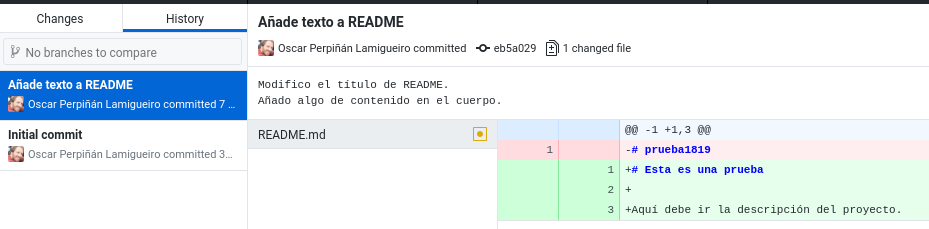
\includegraphics[width=.9\linewidth]{figs/git_history.png}
\end{center}
\end{frame}


\begin{frame}[label={sec:org911cbef},fragile]{Publicar cambios al repositorio remoto}
 \begin{itemize}
\item Para sincronizar  los cambios realizados \alert{desde la copia local hasta el repositorio remoto} hay que publicar mediante \texttt{git push}.
\end{itemize}

\begin{center}
\boxed{Repository > Push}
\end{center}

\begin{itemize}
\item A partir de este punto, la copia local y el repositorio remoto están sincronizados.
\end{itemize}

\begin{block}{Importante}
En el caso de repositorios compartidos, antes de un \texttt{git push} es imprescindible actualizar la copia local incorporando los cambios del repositorio con \texttt{git pull}.
\end{block}
\end{frame}
\begin{frame}[label={sec:org3d74ab4},fragile]{Recibir cambios de un repositorio remoto}
 Para obtener en la copia local los cambios recientes que existan en el repositorio hay que emplear \texttt{git pull}, que es la combinación de la secuencia:
\begin{enumerate}
\item \texttt{git fetch}, para obtener los cambios recientes del repositorio remoto.
\item \texttt{git merge}, para combinarlos con la copia local.
\end{enumerate}

\begin{center}
\boxed{Repository > Pull}
\end{center}
\end{frame}

\begin{frame}[label={sec:org9be598f}]{Resumen}
\begin{enumerate}
\item Realiza modificaciones en los ficheros de la copia local.
\item \alert{COMMIT} :: Confirma los cambios con un mensaje informativo.
\item \alert{PULL} :: Incorpora los cambios del repositorio remoto a la copia local.
\item \alert{PUSH} :: Publica los cambios de la copia local al repositorio remoto.
\end{enumerate}
\end{frame}
\section{Trabajo en colaboración}
\label{sec:org10b621d}
\subsection{Ramas}
\label{sec:org3d2dab0}

\begin{frame}[label={sec:org3644602},fragile]{Rama \texttt{master}}
 \begin{center}
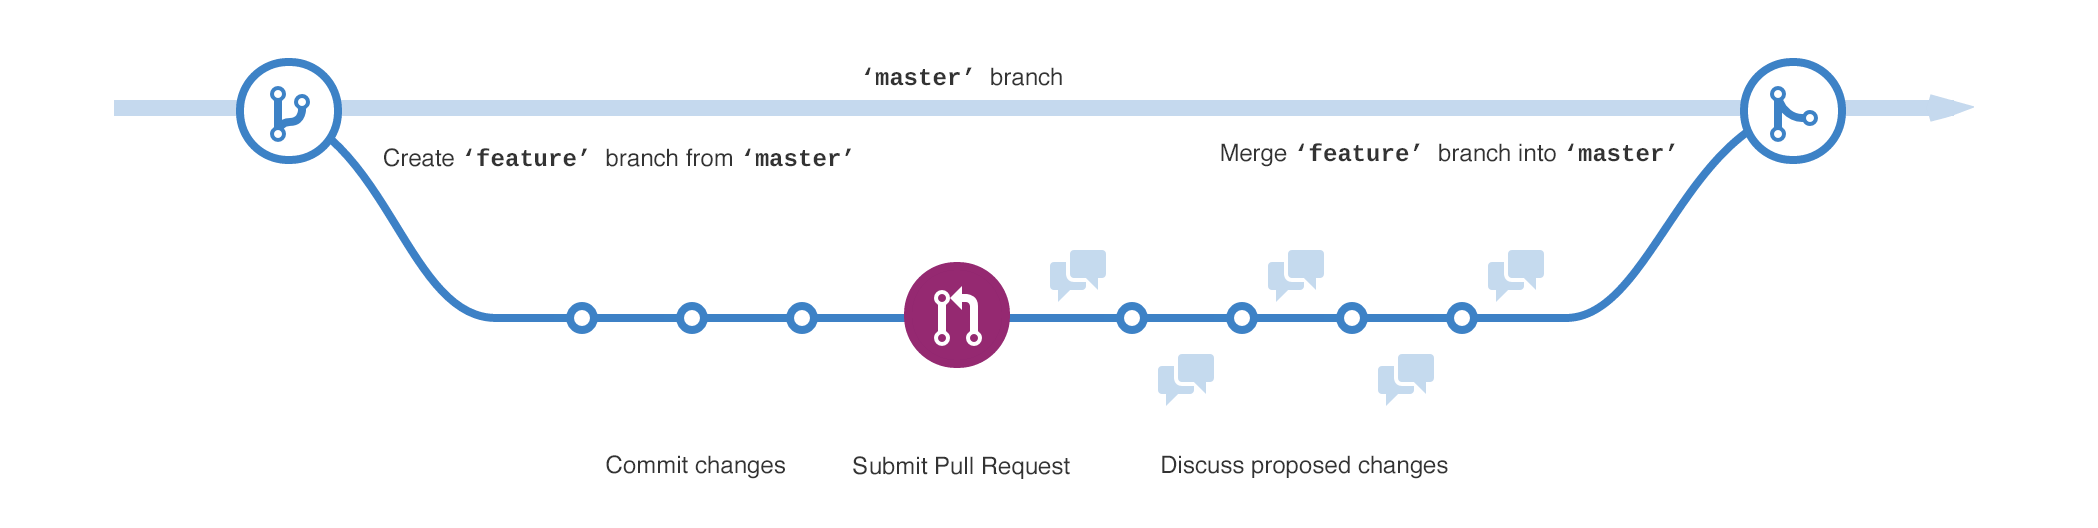
\includegraphics[width=.9\linewidth]{figs/branching.png}
\end{center}

En un repositorio de GitHub existe una rama (\emph{branch}) que se usa por defecto: \alert{master}\footnote{\href{https://guides.github.com/introduction/flow/}{Understanding the GitHub Flow}}.
\end{frame}

\begin{frame}[label={sec:orge925fd5}]{Ramas para facilitar la colaboración}
\begin{center}
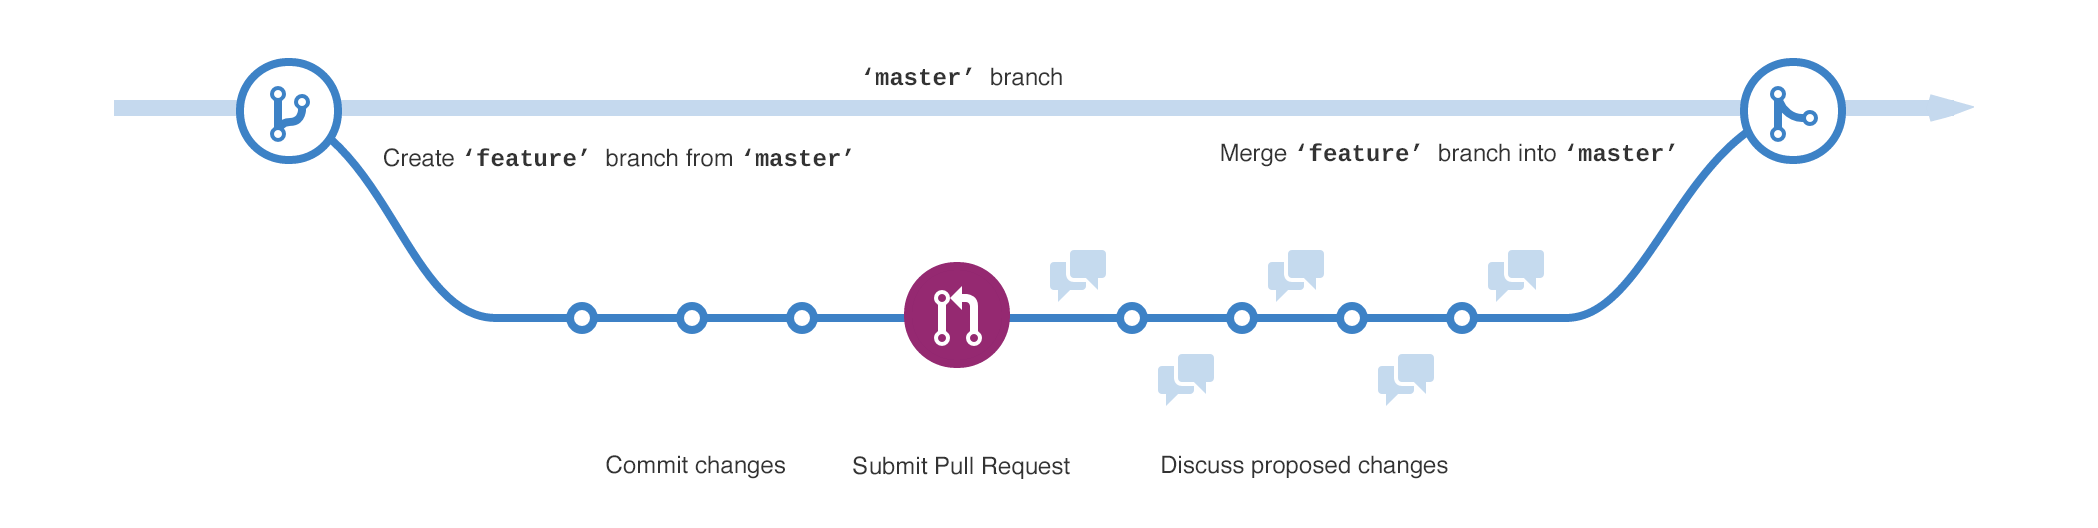
\includegraphics[width=.9\linewidth]{figs/branching.png}
\end{center}

Cuando hay varias personas trabajando sobre un mismo repositorio, es necesario crear nuevas ramas para evitar conflictos. 

De esta forma, cada persona implementa \alert{cambios} en una \alert{rama determinada} de forma paralela al resto del equipo.
\end{frame}

\begin{frame}[label={sec:org1ba2863},fragile]{Crear una nueva rama}
 \begin{itemize}
\item En menú: \boxed{Branch > New\ branch...}

\item O en pantalla principal: \boxed{Current\ branch> Branches > New\ branch}
\end{itemize}

\begin{center}
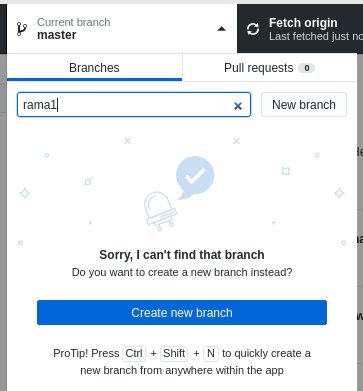
\includegraphics[height=0.5\textheight]{figs/nueva_rama_desktop.png}
\end{center}


La nueva rama puede tener como origen la rama \texttt{master} u otra rama existente.
\end{frame}

\begin{frame}[label={sec:org600eb7a}]{Combinación de código}
\begin{center}
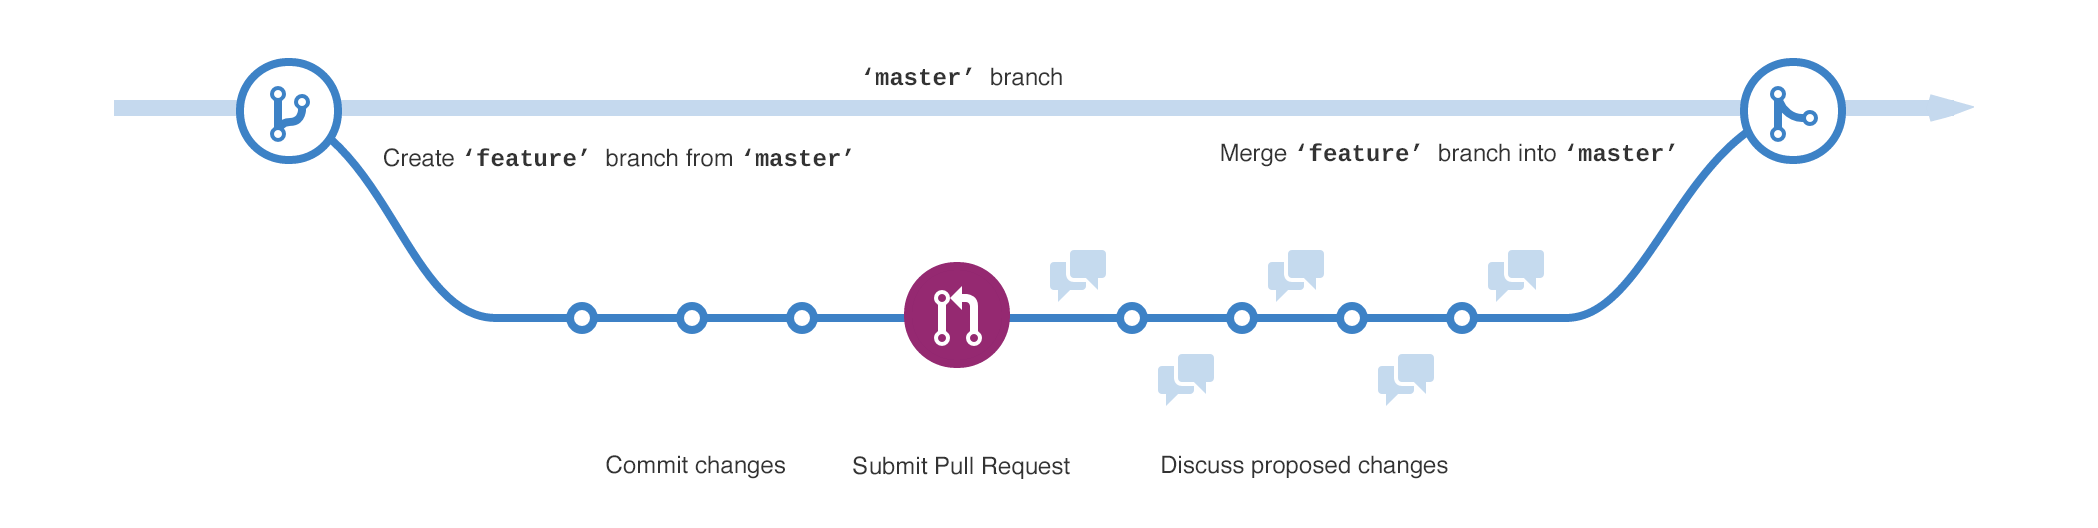
\includegraphics[width=.9\linewidth]{figs/branching.png}
\end{center}

Cuando los cambios están listos y confirmados (\emph{commit} + \emph{push} en la rama específica), se realiza una petición (\emph{pull request}) para combinar estos cambios en la rama \alert{master}.

\begin{columns}
\begin{column}{0.45\columnwidth}
\begin{center}
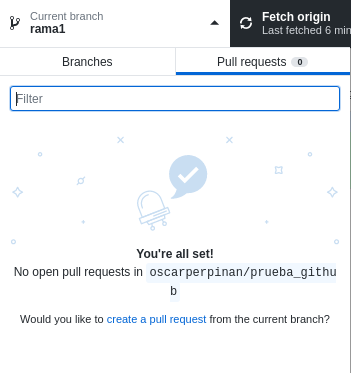
\includegraphics[width=.9\linewidth]{figs/pull_request_desktop.png}
\end{center}
\end{column}

\begin{column}{0.45\columnwidth}
\begin{center}
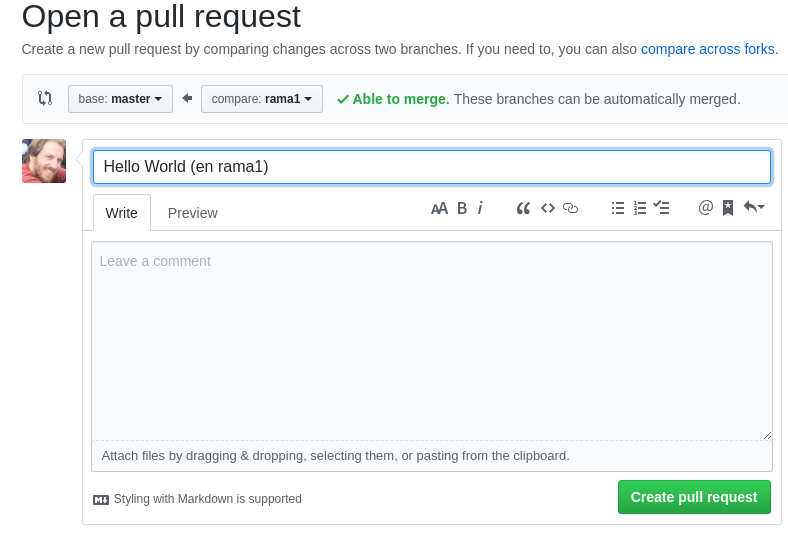
\includegraphics[width=.9\linewidth]{figs/pull_request_web.png}
\end{center}
\end{column}
\end{columns}
\end{frame}

\begin{frame}[label={sec:orgf5bcce5}]{Combinación de código}
\begin{center}
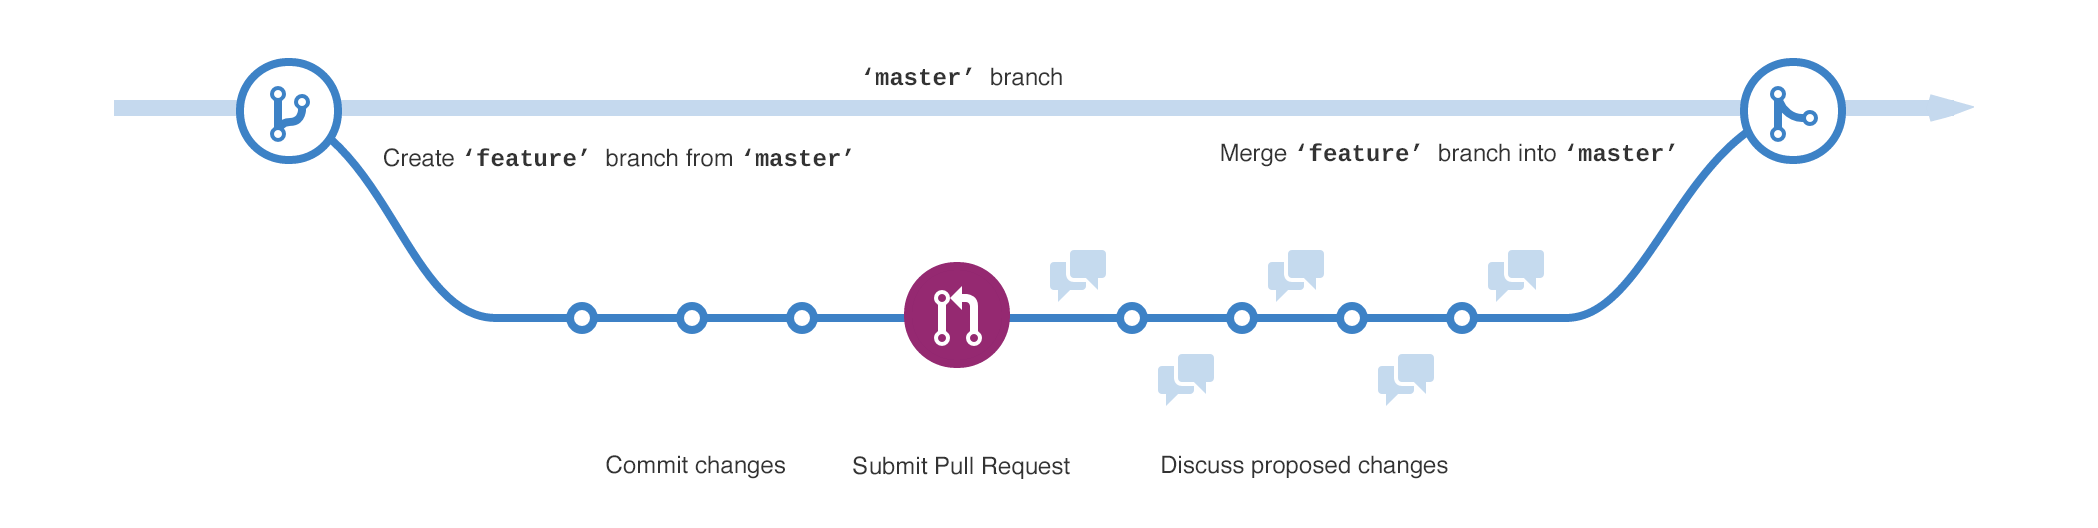
\includegraphics[width=.9\linewidth]{figs/branching.png}
\end{center}


El coordinador del proyecto es el encargado de revisar cada petición y, si todo está correcto, incluir los cambios (\emph{merge}) en la rama \alert{master}. 

\begin{center}
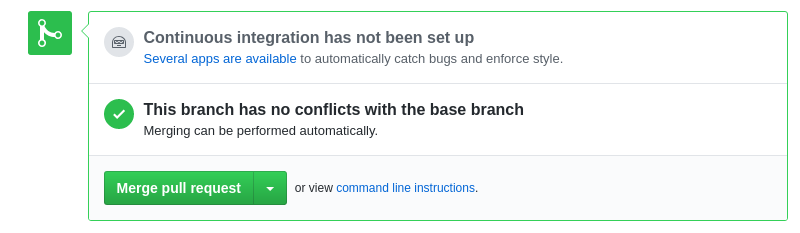
\includegraphics[width=.9\linewidth]{figs/merge_pull_request.png}
\end{center}
\end{frame}

\begin{frame}[label={sec:org60b4869}]{Resolución de conflictos}
Si no se pueden combinar los cambios automáticamente se produce un conflicto (ejemplo: dos usuarios modifican un mismo fichero).

\begin{center}
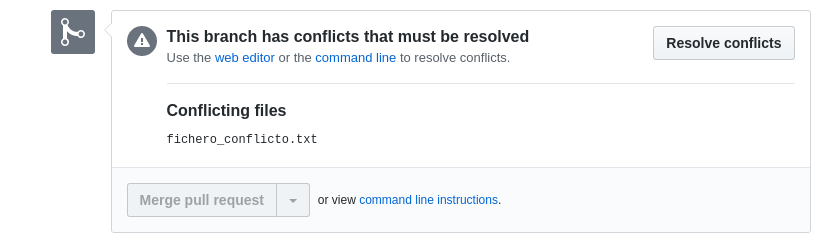
\includegraphics[width=.9\linewidth]{figs/conflict_web.png}
\end{center}

Un conflicto se debe resolver manualmente.
\begin{center}
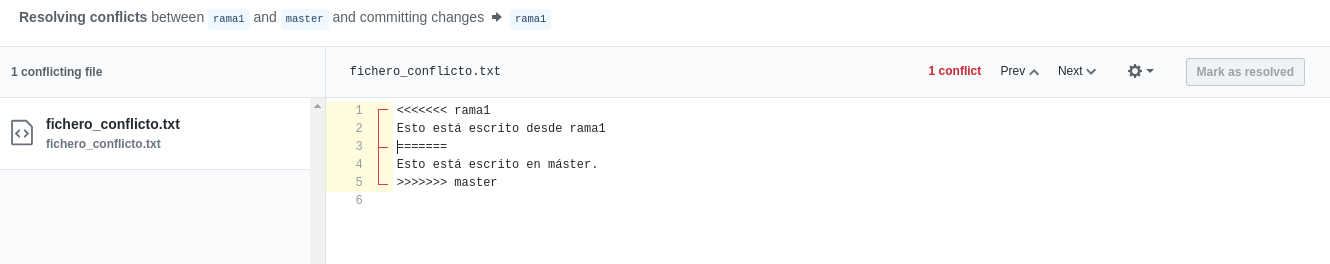
\includegraphics[width=.9\linewidth]{figs/resolve_conflict_web.png}
\end{center}

Lectura recomendada: \href{https://github.blog/2018-08-22-merge-conflicts-in-the-classroom/}{Merge Conflicts in the Classroom}
\end{frame}
\begin{frame}[label={sec:orgb9b7bdd},fragile]{Consejos}
 \begin{itemize}
\item \alert{No olvides hacer \emph{pull} antes de iniciar una nueva interacción con el repositorio}.

\item Recuerda las recomendaciones sobre un buen mensaje de \texttt{git commit}.

\item \alert{Organización previa}: las \alert{tareas} asignadas a un rama deben ser \alert{independientes} de las otras ramas para evitar conflictos.

\item Cuando el trabajo en una rama ha concluido, hay que \alert{combinar cambios con master lo antes posible} para reducir la posibilidad de conflicto. Las ramas accesorias utilizadas se pueden eliminar una vez finalizado el proceso.

\item Este proceso se debe repetir tantas veces como sea necesario para realizar cambios de forma colaborativa.
\end{itemize}
\end{frame}
\begin{frame}[label={sec:org57c33ee},fragile]{}
 \begin{block}{Ejercicio 1}
Crea una nueva rama en tu repositorio. En esta rama crea un nuevo fichero de texto y añade contenido en él. Sincroniza con el repositorio. Vuelve a la rama \texttt{master} y comprueba que este fichero nuevo no está presente. Combina ambas ramas.
\end{block}

\begin{block}{Ejercicio 2}
Vuelve a la rama nueva y modifica un fichero. Vuelve a la rama \texttt{master} y modifica el mismo fichero. Combina ambas ramas y resuelve los conflictos.
\end{block}
\end{frame}
\subsection{Persiguiendo a los bichos}
\label{sec:org00bf963}

\begin{frame}[label={sec:org4709516}]{Issues}
Todos los repositorios de GitHub tienen una sección denominada \guillemotleft{}Issues\guillemotright{}\footnote{\url{https://guides.github.com/features/issues/}} a modo de \emph{bug tracker}.

Pueden usarse para seguimiento de fallos, mejoras, tareas, etc.

\begin{center}
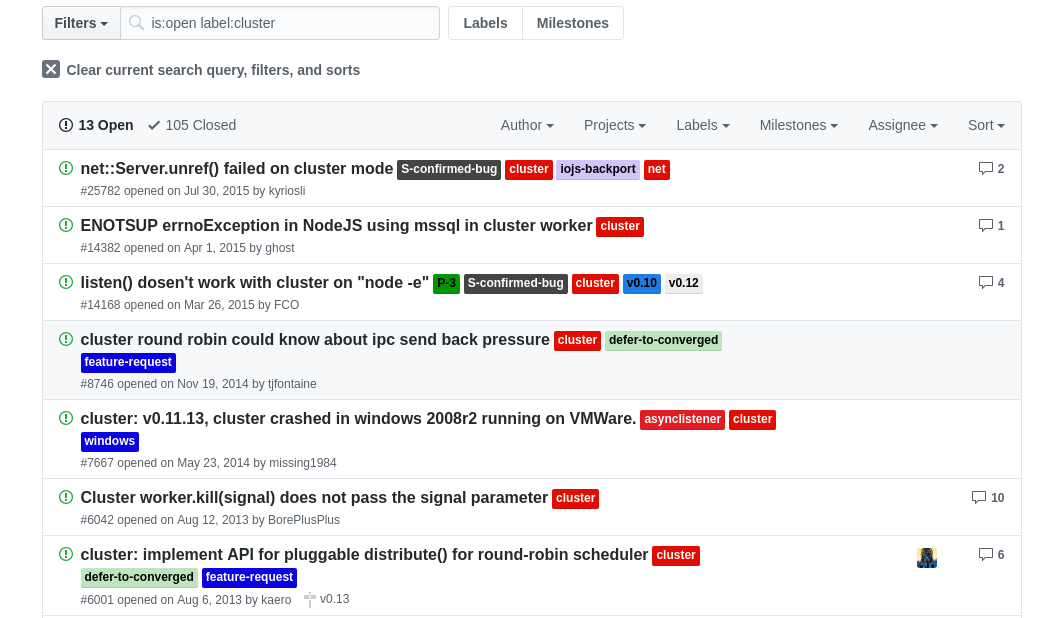
\includegraphics[width=.9\linewidth]{figs/github_issues.png}
\end{center}
\end{frame}

\begin{frame}[label={sec:orgbbc7b64}]{Estructura de una issue}
Una issue es un tablero de discusión en el que pueden participar los responsables del repositorio y cualquier usuario de GitHub.

\alert{Debe} contener un título y una descripción.

\alert{Puede} contener etiquetas, metas, y responsables.

\begin{center}
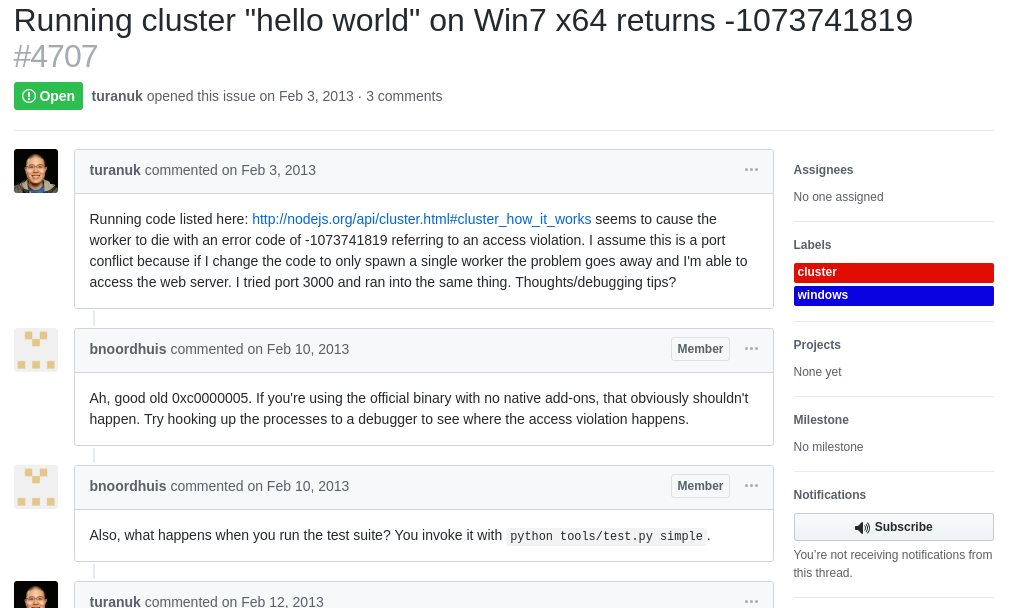
\includegraphics[width=.9\linewidth]{figs/github_issue_example.png}
\end{center}
\end{frame}

\begin{frame}[label={sec:orgdadb63a}]{Contenido de una issue}
\begin{itemize}
\item En la descripción de una issue se debe suministrar toda la información posible para el responsable del repositorio, \alert{incluyendo un ejemplo mínimo, completo y verificable}\footnote{\url{https://stackoverflow.com/help/mcve}}.

\item El contenido será formateado como Markdown (incluye un \emph{preview})\footnote{Veáse la guía \href{https://help.github.com/articles/basic-writing-and-formatting-syntax/}{Basic Writing and Formatting syntax}.}.

\item Se pueden incluir referencias al código y a otras issues\footnote{Veáse la guía \href{https://help.github.com/articles/autolinked-references-and-urls/}{Autolinked references and urls}.}.
\end{itemize}
\end{frame}

\begin{frame}[label={sec:org23341e9},fragile]{}
 \begin{block}{Ejercicio}
\begin{itemize}
\item Abre nuevas \texttt{issues} en tu propio repositorio, o en repositorios ajenos (por ejemplo, \url{https://github.com/oscarperpinan/prueba\_github}).

\item Responde y cierra \texttt{issues} de otros usuarios en tu propio repositorio.
\end{itemize}
\end{block}
\end{frame}

\subsection{Herramientas gráficas para el análisis de un repositorio}
\label{sec:org1bc3b09}

\begin{frame}[label={sec:org020a44b}]{Insights}
Toda la actividad realizada en un repositorio puede verse de manera gráfica a través del botón \emph{Insights} en la web del repositorio en GitHub\footnote{Más detalles en \href{https://help.github.com/categories/visualizing-repository-data-with-graphs/}{Ver información del repositorio de forma gráfica}.}. Por ejemplo,

\begin{itemize}
\item Contribución de los integrantes del equipo
\item Estructuras de ramas de un repositorio
\item Histórico de cambios en un repositorio
\end{itemize}
\end{frame}

\begin{frame}[label={sec:orgc87d485}]{Contribución de los integrantes del equipo}
\begin{center}
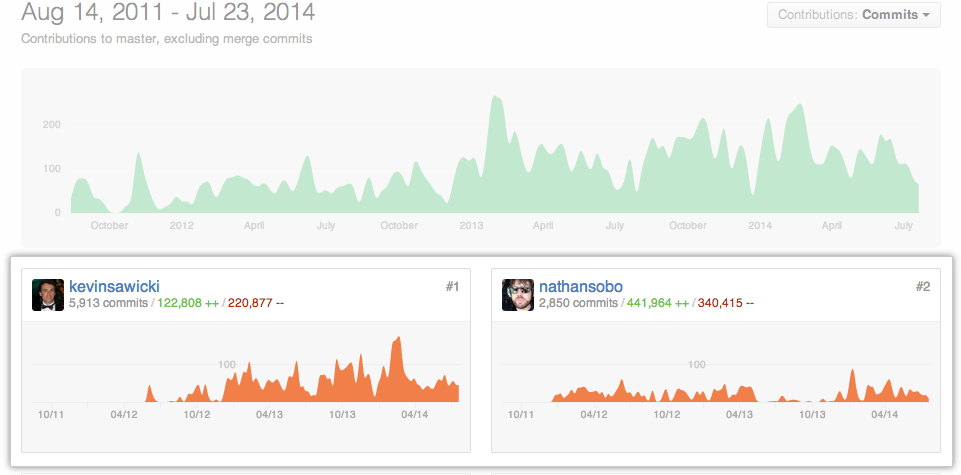
\includegraphics[width=.9\linewidth]{figs/repo_contributors_specific_graph.png}
\end{center}
\end{frame}

\begin{frame}[label={sec:org6849170}]{Estructura de ramas de un repositorio}
\begin{center}
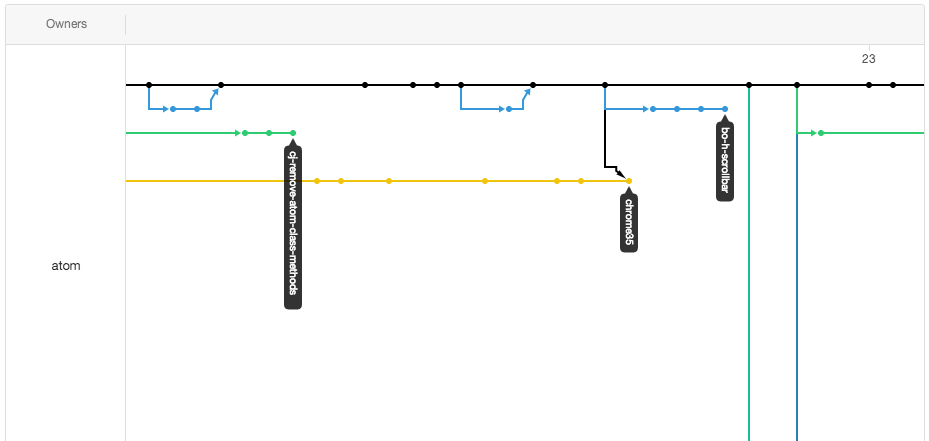
\includegraphics[width=.9\linewidth]{figs/repo_network_graph.png}
\end{center}
\end{frame}

\begin{frame}[label={sec:org537fcf1}]{Cambios en un repositorio}
\begin{center}
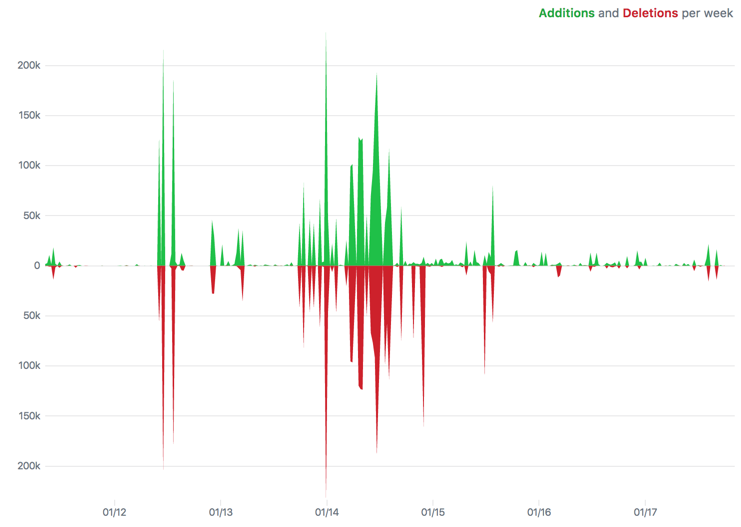
\includegraphics[width=.9\linewidth]{figs/repo_code_frequency_graph_dotcom.png}
\end{center}
\end{frame}

\begin{frame}[label={sec:orgb3c2b0e}]{}
\begin{block}{Ejercicio}
Visita la sección Insights de los repositorios del proyecto AIGORA (\url{https://github.com/aigora}). 

Por ejemplo: \url{https://github.com/aigora/twE105-cafranpa}
\end{block}
\end{frame}

\section{GitHub Classroom}
\label{sec:org5d04e3c}

\begin{frame}[label={sec:org0c17fe7}]{¿Qué es GitHub Classroom?}
\begin{itemize}
\item Es un asistente para configurar grupos y asignar tareas en GitHub. Accesible en: \url{https://classroom.github.com/}

\item Es recomendable \href{https://help.github.com/en/articles/applying-for-an-educator-or-researcher-discount}{solicitar descuento por cuenta académica} (repositorios públicos y privados ilimitados, colaboradores ilimitados).
\end{itemize}
\end{frame}


\begin{frame}[label={sec:orgfee8f47},fragile]{GitHub Classroom necesita una Organización}
 \begin{itemize}
\item Para poder trabajar con GitHub Classroom es necesario crear una Organización en Github (grupo de cuentas que tienen acceso compartido a un grupo de repositorios): \url{https://github.com/organizations/new}

\item Ejemplo: \url{https://github.com/swcarpentry}

\item Dentro de una \texttt{organization} pueden coexistir diferentes equipos (\texttt{Team}), cada uno de ellos con diferentes permisos de acceso y escritura a los repositorios.

\item Las cuentas tipo \texttt{organization} también pueden solicitar el \href{https://help.github.com/en/articles/applying-for-an-educator-or-researcher-discount\#upgrading-your-organization}{descuento por cuenta académica}.

\item Más información en el \href{https://github.blog/2010-06-29-introducing-organizations/}{blog de GitHub}.
\end{itemize}
\end{frame}

\begin{frame}[label={sec:org7ed5c64},fragile]{Configuración de aulas y tareas}
 \begin{itemize}
\item Una única cuenta \texttt{organization} puede dar cabida a múltiples aulas (\texttt{classrooms}): \url{https://classroom.github.com/classrooms/}
\item Dentro de cada \texttt{classroom} se pueden incluir múltiples tareas (\texttt{assignments}).
\item Un \texttt{assignment} puede ser individual o grupal (los grupos se pueden definir antes por el profesor, o por los estudiantes en el momento de aceptar la tarea.)
\item Cada \texttt{classroom} contiene estudiantes (identificados por su usuario de GitHub y su correo electrónico) y grupos (\texttt{teams}).
\item Esta correspondencia se puede facilitar mediante el \texttt{classroom roster}.
\end{itemize}
\end{frame}

\begin{frame}[label={sec:org6761d50},fragile]{Cómo hemos usado GitHub Classroom en AIGORA}
 \begin{block}{Configuración General}
\begin{itemize}
\item Usamos una \texttt{organization} común para todos los grupos de matriculación de una misma asignatura.
\item Definimos un \texttt{classroom} para cada grupo de matriculación.
\item En cada \texttt{classroom} subimos la lista de correos UPM de los estudiantes de ese grupo de matriculación mediante el \texttt{roster management}.
\item Dentro de cada \texttt{classroom} definimos diferentes equipos de trabajo (\texttt{Teams}) para trabajos grupales.
\end{itemize}
\end{block}
\end{frame}
\begin{frame}[label={sec:org66e4c2a},fragile]{Cómo hemos usado GitHub Classroom en AIGORA}
 \begin{block}{Registro de estudiantes}
\begin{enumerate}
\item En cada \texttt{classroom} creamos una \texttt{Group Assignment} denominada \guillemotleft{}registro estudiantes\guillemotright{}. Como identificador del \guillemotleft{}Group\guillemotright{} utilizamos el grupo de matriculación. Este identificador queda almacenado en GitHub Classroom para futuros usos, pero \alert{no} crea un \texttt{Team} en GitHub.
\item Abrimos el enlace del assignment con nuestro usuario (podemos hacer \texttt{skip} cuando nos pide que enlacemos a algún miembro del \texttt{roster}), y \alert{creamos un nuevo Team}, que se debe llamar igual que el grupo de matriculación. Este paso \alert{sí} crea un nuevo \texttt{Team} en la organization de Github (útil para asignar permisos grupales).
\item A continuación enviamos el enlace del \texttt{assignment} a los alumnos para que enlacen su usuario de GitHub a su correo incluido en el roster.  \alert{Deben elegir el Team que hemos definido nosotros, sin crear uno nuevo}. A partir de este punto forman parte del \texttt{Team} con los permisos y repositorios definidos para el mismo.
\end{enumerate}
\end{block}
\end{frame}
\begin{frame}[label={sec:orga7938a5},fragile]{Cómo hemos usado GitHub Classroom en AIGORA}
 \begin{block}{Grupos de Trabajo}
\begin{enumerate}
\item Para el trabajo en equipo creamos igualmente una \texttt{Group Assignment}, pero dejamos libertad a la hora de definir los \texttt{Teams}.
\item El primer estudiante de un grupo de trabajo que acepta este \texttt{assignment} define el nombre del \texttt{Team}. Los siguientes estudiantes de ese mismo grupo deben seleccionar ese \texttt{Team}.
\item Se pueden definir repositorios plantilla para incluir contenido inicial en todos los repositorios creados para cada \texttt{Team}. Ejemplo: \url{https://github.com/aigora/starter-code}
\end{enumerate}
\end{block}
\end{frame}

\section{Publicación de páginas web en GitHub}
\label{sec:orgcb46848}

\begin{frame}[label={sec:org16b4a2c},fragile]{Página web de \alert{proyecto}}
 \begin{block}{Si no sabes HTML}
\begin{itemize}
\item En la página del repositorio:
\end{itemize}

\begin{center}
\boxed{Settings > GitHub\ Pages > Source > master\ branch}

\boxed{Settings > GitHub\ Pages > Theme\ Chooser}
\end{center}

\begin{itemize}
\item Modifica el fichero \texttt{README.md}\footnote{Más información sobre formato Markdown \url{https://guides.github.com/features/mastering-markdown/}.} (\texttt{commit} + \texttt{push}).

\item Con un navegador ve a la dirección \url{https://<username>.github.io/<repository>}
\end{itemize}
\end{block}
\end{frame}

\begin{frame}[label={sec:org64863cc},fragile]{Página web de \alert{proyecto}}
 \begin{block}{Si sabes HTML}
\begin{itemize}
\item Crea una carpeta \texttt{docs} en la rama \texttt{master} del repositorio.

\item En esta carpeta \texttt{docs} crea/modifica un fichero \texttt{index.html} (\texttt{commit} + \texttt{push}).

\item En la página del repositorio:
\end{itemize}

\begin{center}
\boxed{Settings > GitHub\ Pages > Source > docs\ folder}
\end{center}

\begin{itemize}
\item Con un navegador ve a la dirección \url{https://<username>.github.io/<repository>}
\end{itemize}
\end{block}
\end{frame}
\begin{frame}[label={sec:org227a6d9}]{Ejemplo de web de \alert{proyecto}}
\begin{itemize}
\item Página web: \url{https://oscarperpinan.github.io/bookvis/}
\item Repositorio: \url{https://github.com/oscarperpinan/bookvis/tree/master/docs}
\end{itemize}

\begin{center}
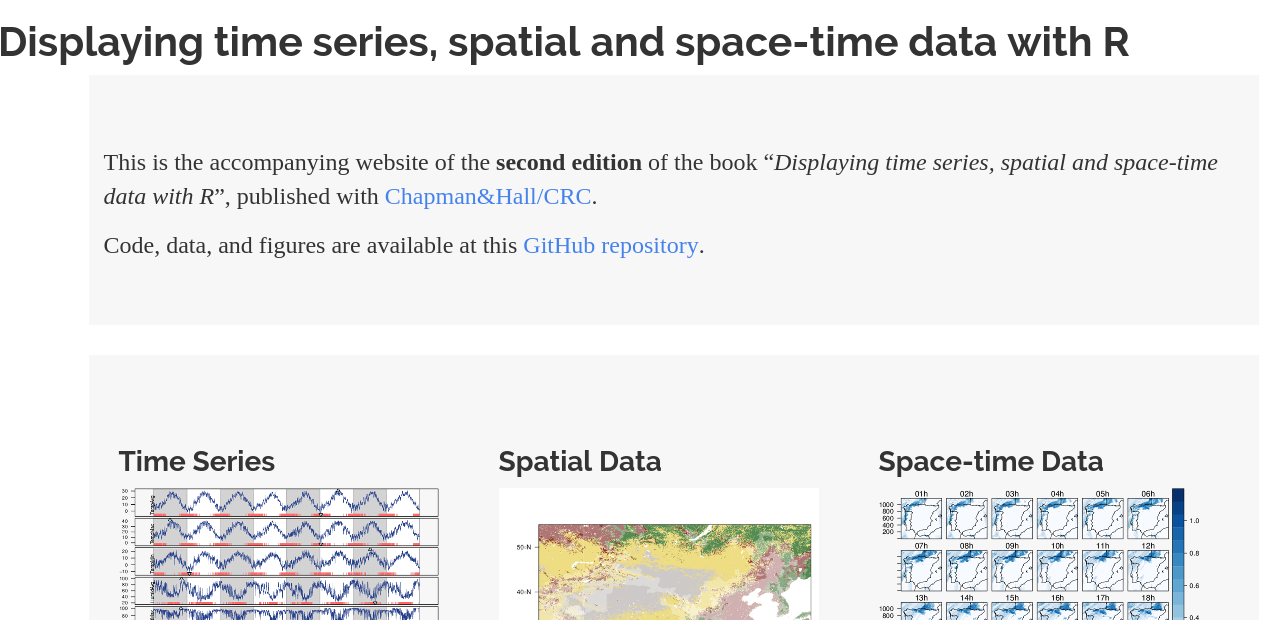
\includegraphics[width=.9\linewidth]{figs/captura_bookvis.png}
\end{center}
\end{frame}


\begin{frame}[label={sec:orge4448d9},fragile]{Página web de \alert{usuario u organización}}
 \begin{enumerate}
\item Crea un repositorio nuevo con el nombre \texttt{<username>.github.io}\footnote{Siendo \texttt{<username>} tu nombre de usuario en GitHub.}.
\item Sube (\texttt{commit} + \texttt{push}) un fichero \texttt{index.html} a la rama \texttt{master} con código HTML.
\item Con un navegador ve a la dirección \url{https://<username>.github.io}
\end{enumerate}

\lstset{language=HTML,label= ,caption= ,captionpos=b,numbers=none}
\begin{lstlisting}
<!DOCTYPE HTML>
<html>
	<head>
		<title>Hello World</title>
	</head>
	<body>
		Hello World!
	</body>
</html>
\end{lstlisting}
\end{frame}

\begin{frame}[label={sec:org5d5bd1a}]{Ejemplo de web de \alert{organización}}
\begin{itemize}
\item Página web: \url{https://aigora.github.io/}
\item Repositorio: \url{https://github.com/aigora/aigora.github.io}
\end{itemize}


\begin{center}

\includegraphics[width=.9\linewidth]{figs/captura_aigora.png}
\end{center}
\end{frame}
\end{document}